\documentclass[border=6pt]{standalone}
\usepackage{amsmath}
\usepackage{tikz}
\usetikzlibrary{arrows.meta}
\begin{document}
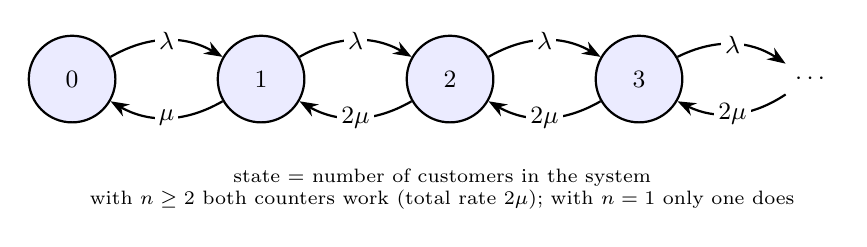
\begin{tikzpicture}[>=Stealth,font=\small,
 s/.style={draw,thick,circle,minimum size=1.1cm,inner sep=0pt,fill=blue!8},
 e/.style={->,thick},
 lab/.style={font=\small,fill=white,inner sep=1.5pt},
 every loop/.style={->,thick,looseness=6}]
\node[s] (0) at (0,0) {$0$};
\node[s] (1) at (2.4,0) {$1$};
\node[s] (2) at (4.8,0) {$2$};
\node[s] (3) at (7.2,0) {$3$};
\node (d) at (9.4,0) {$\cdots$};
\foreach \a/\b/\m in {0/1/\mu,1/2/2\mu,2/3/2\mu,3/d/2\mu} {
  \draw[e] (\a) to[bend left=30] node[lab]{$\lambda$} (\b);
  \draw[e] (\b) to[bend left=30] node[lab]{$\m$} (\a);
}
\node[font=\scriptsize,align=center] at (4.7,-1.4) {state = number of customers in the system\\with $n\ge2$ both counters work (total rate $2\mu$); with $n=1$ only one does};
\end{tikzpicture}
\end{document}
